\chapter{Results}
\label{Results}
\section{Experiment Description}
To demonstrate our results, we plotted results from one standardized run of multiple division configurations trained over 2'000 rounds of 10'000 hands each, for a total of 20'000'000 hands.

All divisions included one random and one call agent as baselines, and all divisions cloned a new generation of teachers every 200 rounds, for a total of 90 agents over the whole run.

\begin{table}[h!]
\centering
\begin{tabular}{|| c | c | c ||} 
 \hline
 Name & Matchup Method & Agents \\ [0.5ex] 
 \hline\hline
 Qln8-Cl & Climbing & Qlearn-8 \\
 QlnA-Cl & Climbing & Qlearn-All \\
 SacL-Cl & Climbing & Sac-Low \\
 SacH-Cl & Climbing & Sac-High \\
 AllAg-Cl & Climbing & Qlearn-8, Qlearn-All, Sac-Low, Sac-High \\
 QlnA-Rn & Random & Qlearn-All \\ [1ex] 
 \hline
\end{tabular}
\caption{Training division configurations used in the standardized run}
\label{RunDivisions}
\end{table}

We trained on a computer with an Intel 6770k CPU, 16GB Ram, and an Nvidia 1070GTX GPU with 8GB VRAM. The training process took about 44 hours in real-time.

After training, we ran three PermaEval divisions to evaluate all agents according to the various metrics: one for all the winnings-based metrics, one for across-division TrueSkill, and a second TrueSkill to evaluate its consistency.

We computed winnings with 10'000 hands per agent pairing of all 102 agents, for a total of 52'020'000 hands. For fairness of comparison, TrueSkill was evaluated for the same number of rounds.

\section{Performance Metrics}

\subsection{Leaderboards}

\begin{table}[H]
\centering
\subcaptionbox{Sorted by TrueSkill (TS)}{
\begin{tabular}{|| c | c | c | c | c ||} 
 \hline
 Name & TS & Mean & Med & 20-Pctl \\ [0.5ex] 
 \hline\hline
     exam &     151.24 &  3.26 &    2.35 &           0.21 \\
     loss &     147.96 &  3.95 &    2.76 &           0.33 \\
    radar &     146.88 &  2.79 &    2.02 &           0.14 \\
      tan &     144.55 &  4.47 &    2.55 &           0.19 \\
    brick &     143.52 &  5.13 &    2.65 &           0.35 \\
     clam &     143.26 &  4.67 &    2.81 &           0.15 \\
   seeker &     141.63 &  6.16 &    2.98 &           0.33 \\
   flight &     139.47 &  4.58 &    2.53 &           0.23 \\
 suitcase &     139.11 &  4.81 &    2.45 &           0.33 \\
   wisdom &     138.66 &  1.47 &    0.94 &           0.06 \\ [1ex] 
 \hline
\end{tabular}
}
\subcaptionbox{Sorted by Mean
}{
\begin{tabular}{|| c | c | c | c | c ||} 
 \hline
 Name & TS & Mean & Med & 20-Pctl \\ [0.5ex] 
 \hline\hline
   orange &     130.47 &  6.79 &    1.32 &          -0.07 \\
     watt &     133.64 &  6.59 &    2.24 &           0.23 \\
   seeker &     141.63 &  6.16 &    2.98 &           0.33 \\
 ecclesia &     124.43 &  6.15 &    1.42 &           0.00 \\
   config &     122.03 &  6.06 &    0.89 &          -1.20 \\
    power &     131.36 &  6.04 &    1.58 &           0.00 \\
  creator &     136.04 &  5.91 &    2.59 &           0.03 \\
    union &     131.07 &  5.65 &    1.50 &           0.01 \\
  cowbell &     117.96 &  5.50 &    0.88 &          -2.32 \\
     yarn &     119.87 &  5.50 &    1.14 &          -1.60 \\ [1ex] 
 \hline
\end{tabular}
}
\subcaptionbox{Sorted by Median (Med)
}{
\begin{tabular}{|| c | c | c | c | c ||} 
 \hline
 Name & TS & Mean & Med & 20-Pctl \\ [0.5ex] 
 \hline\hline
   seeker &     141.63 &  6.16 &    2.98 &           0.33 \\
     clam &     143.26 &  4.67 &    2.81 &           0.15 \\
  penguin &     135.57 &  5.22 &    2.76 &           0.00 \\
     loss &     147.96 &  3.95 &    2.76 &           0.33 \\
    brick &     143.52 &  5.13 &    2.65 &           0.35 \\
  creator &     136.04 &  5.91 &    2.59 &           0.03 \\
      tan &     144.55 &  4.47 &    2.55 &           0.19 \\
   flight &     139.47 &  4.58 &    2.53 &           0.23 \\
 suitcase &     139.11 &  4.81 &    2.45 &           0.33 \\
     exam &     151.24 &  3.26 &    2.35 &           0.21 \\[1ex] 
 \hline
\end{tabular}
}
\subcaptionbox{Sorted by 20-Percentile (20-Pctl)
}{
\begin{tabular}{|| c | c | c | c | c ||} 
 \hline
 Name & TS & Mean & Med & 20-Pctl \\ [0.5ex] 
 \hline\hline
    brick &     143.52 &  5.13 &    2.65 &           0.35 \\
 suitcase &     139.11 &  4.81 &    2.45 &           0.33 \\
     loss &     147.96 &  3.95 &    2.76 &           0.33 \\
   seeker &     141.63 &  6.16 &    2.98 &           0.33 \\
     watt &     133.64 &  6.59 &    2.24 &           0.23 \\
   flight &     139.47 &  4.58 &    2.53 &           0.23 \\
     exam &     151.24 &  3.26 &    2.35 &           0.21 \\
      tan &     144.55 &  4.47 &    2.55 &           0.19 \\
     rain &     134.44 &  4.20 &    1.01 &           0.17 \\
     clam &     143.26 &  4.67 &    2.81 &           0.15 \\[1ex] 
 \hline
\end{tabular}
}
\label{TopAgentsMetrics}
\caption{Top 10 agents sorted by each metric}
\end{table}

\begin{table}[H]
\centering
\begin{tabular}{|| c | c ||} 
 \hline
 Metric & \% Upsets \\ [0.5ex] 
 \hline\hline
    TrueSkill & 1 \\
    Mean & 1 \\
    Median & 1 \\
    20-Percentile & 1 \\ [1ex]
 \hline
\end{tabular}
\label{MetricsUpsets}
\caption{\% Upsets per metric}
\end{table}

\begin{code}
    -discussion
    -correlation (kendall-tau)
    -sorting by n upsets
\end{code}

\begin{figure}[H]
\centering
\subcaptionbox{
    Colored by TrueSkill
}{
    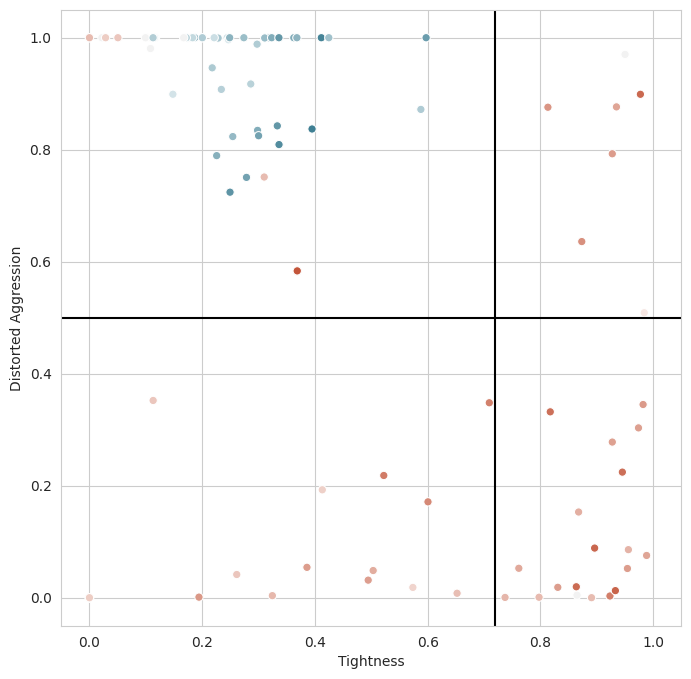
\includegraphics[width=0.45\linewidth]{Results/figures/aggtightrankTrueSkill.png}
}
\subcaptionbox{
    Colored by Mean
}{
    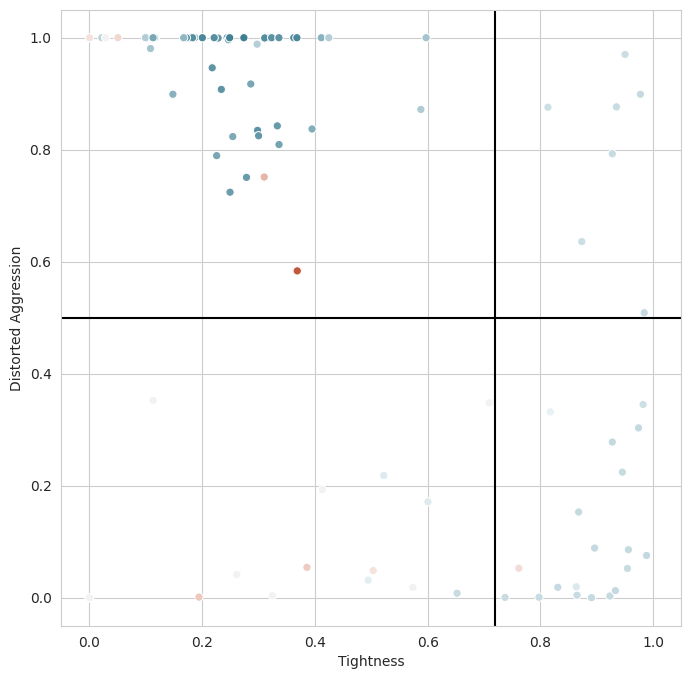
\includegraphics[width=0.45\linewidth]{Results/figures/aggtightrankMean.png}
}
\subcaptionbox{
    Colored by Median
}{
    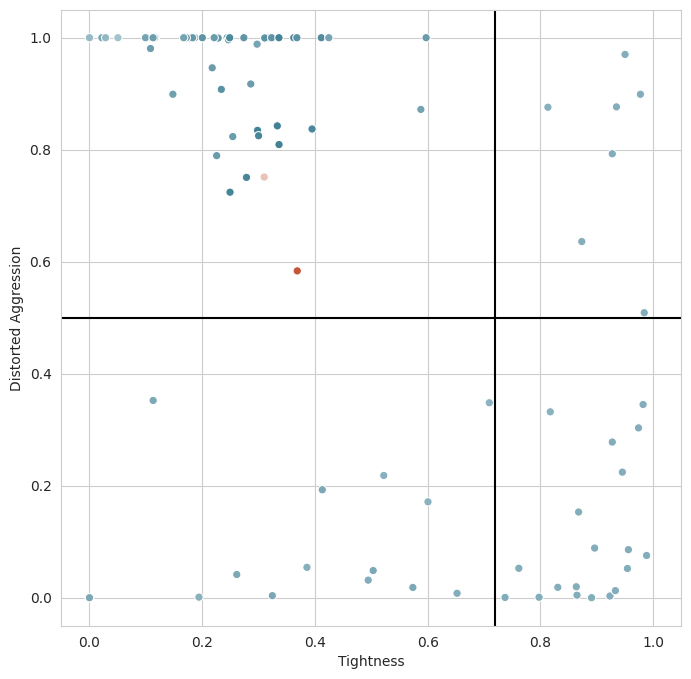
\includegraphics[width=0.45\linewidth]{Results/figures/aggtightrankMedian.png}
}
\subcaptionbox{
    Colored by 20-Percentile
}{
    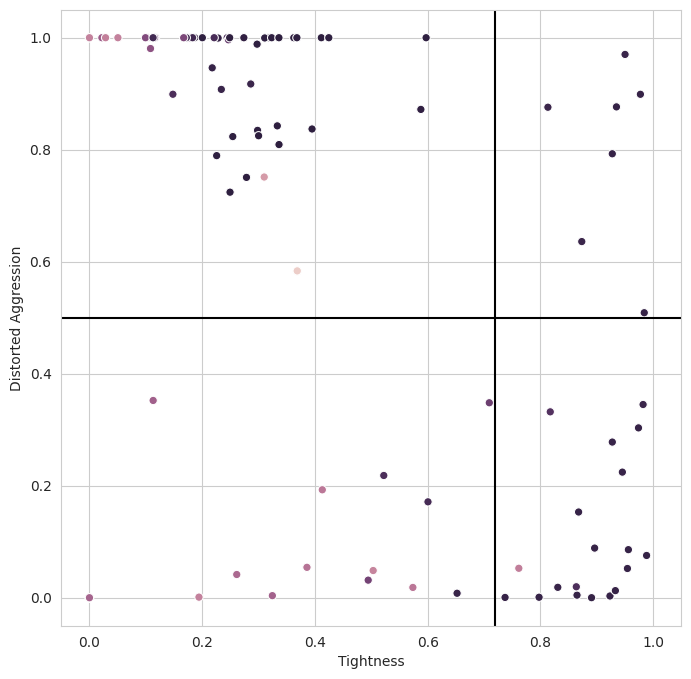
\includegraphics[width=0.45\linewidth]{Results/figures/aggtightrank20-Percentile.png}
}
\caption{Aggression and Tightness colored by rank for each metric}
\label{AggTightRank}
\end{figure}

\begin{code}
    -discussion
\end{code}

\subsection{TrueSkill Coherence}
\begin{figure}[H]
\centering
\subcaptionbox{
    TrueSkill over time in the first PermaEval division
}{
    
\includegraphics[width=\linewidth]{Results/figures/placeholder.png}
}
\subcaptionbox{
    TrueSkill over time in the second PermaEval division
}{
    
\includegraphics[width=\linewidth]{Results/figures/placeholder.png}
}
\caption{TrueSkill over time in both PermaEval divisions, compared}
\label{TrueSkillCompare}
\end{figure}
\begin{code}
    - discussion
\end{code}
\begin{figure}[H]
\centering
    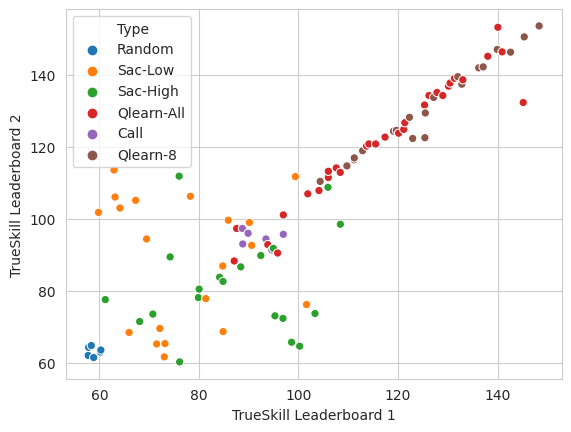
\includegraphics[width=0.8\linewidth]{Results/figures/trueskill_comparison.png}
\caption{Agent rank in both TrueSkill PermaEval divisions}
\label{TrueSkillCompare2}
\end{figure}
\begin{code}
    - (kendall-tau)
    - trueskill bad
\end{code}

\section{Agents}
\begin{table}[H]
\centering
\begin{tabular}{|| c | c | c | c | c | c ||} 
 \hline
 Rank & TrueSkill & Mean & Median & 20-Percentile \\ [0.5ex] 
 \hline\hline
   1 &    Qlearn-8 &  Qlearn-All &  Qlearn-All &    Qlearn-All \\
   2 &    Qlearn-8 &  Qlearn-All &    Qlearn-8 &    Qlearn-All \\
   3 &  Qlearn-All &  Qlearn-All &    Qlearn-8 &      Qlearn-8 \\
   4 &    Qlearn-8 &  Qlearn-All &    Qlearn-8 &      Qlearn-8 \\
   5 &  Qlearn-All &  Qlearn-All &  Qlearn-All &    Qlearn-All \\
   6 &    Qlearn-8 &  Qlearn-All &  Qlearn-All &      Qlearn-8 \\
   7 &  Qlearn-All &  Qlearn-All &    Qlearn-8 &      Qlearn-8 \\
   8 &    Qlearn-8 &  Qlearn-All &    Qlearn-8 &      Qlearn-8 \\
   9 &    Qlearn-8 &  Qlearn-All &    Qlearn-8 &    Qlearn-All \\
  10 &  Qlearn-All &  Qlearn-All &    Qlearn-8 &      Qlearn-8 \\
  11 &  Qlearn-All &  Qlearn-All &  Qlearn-All &    Qlearn-All \\
  12 &    Qlearn-8 &  Qlearn-All &  Qlearn-All &    Qlearn-All \\
  13 &  Qlearn-All &    Qlearn-8 &  Qlearn-All &      Qlearn-8 \\
  14 &    Qlearn-8 &  Qlearn-All &    Qlearn-8 &    Qlearn-All \\
  15 &  Qlearn-All &    Qlearn-8 &  Qlearn-All &    Qlearn-All \\
  16 &  Qlearn-All &    Qlearn-8 &    Qlearn-8 &      Qlearn-8 \\
  17 &  Qlearn-All &    Qlearn-8 &  Qlearn-All &    Qlearn-All \\
  18 &  Qlearn-All &    Qlearn-8 &  Qlearn-All &    Qlearn-All \\
  19 &    Qlearn-8 &    Qlearn-8 &  Qlearn-All &    Qlearn-All \\
  20 &  Qlearn-All &    Qlearn-8 &  Qlearn-All &    Qlearn-All \\[1ex] 
 \hline
\end{tabular}
\label{TypeRankings}
\caption{Agent type of the top 20 agents according to each metric}
\end{table}

\begin{figure}[H]
\centering
\subcaptionbox{
    Ranked by TrueSkill
}{
    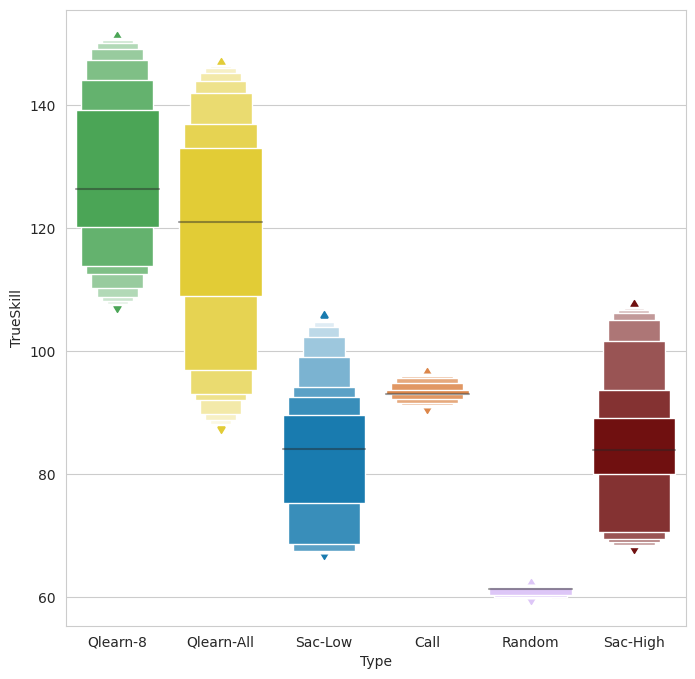
\includegraphics[width=0.45\linewidth]{Results/figures/agentdistTrueSkill.png}
}
\subcaptionbox{
    Ranked by Mean
}{
    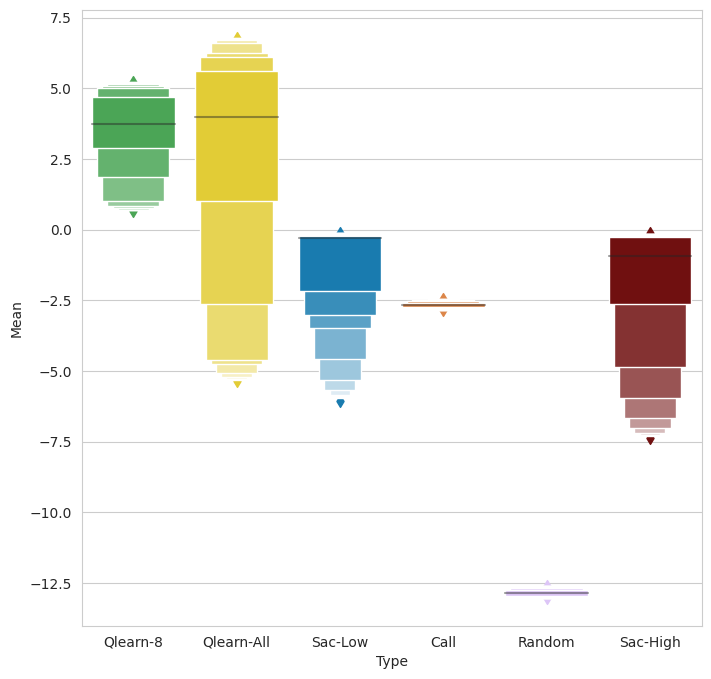
\includegraphics[width=0.45\linewidth]{Results/figures/agentdistMean.png}
}
\subcaptionbox{
    Ranked by Median
}{
    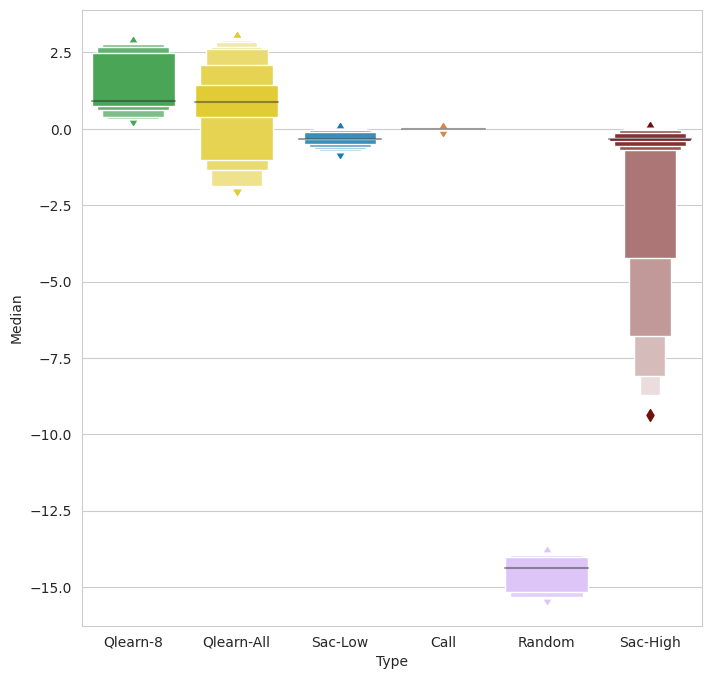
\includegraphics[width=0.45\linewidth]{Results/figures/agentdistMedian.png}
}
\subcaptionbox{
    Ranked by 20-Percentile
}{
    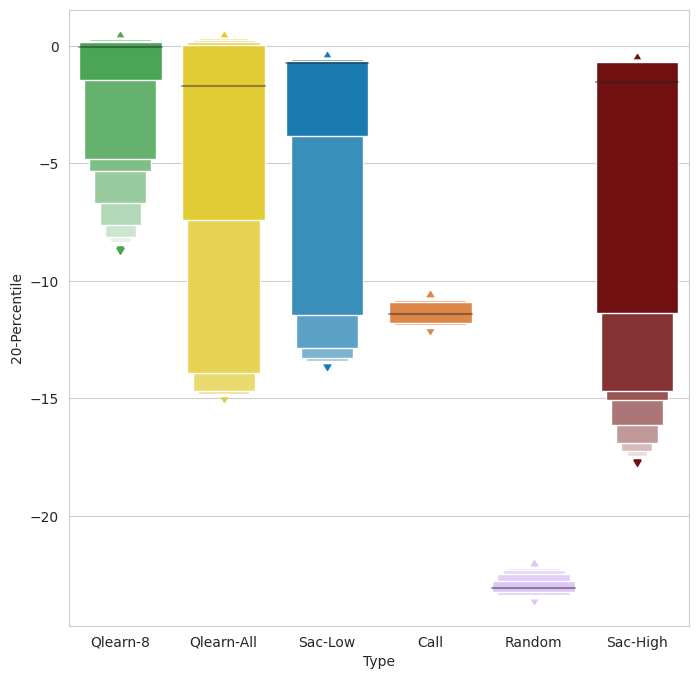
\includegraphics[width=0.45\linewidth]{Results/figures/agentdist20-Percentile.png}
}
\caption{Agent distribution by type and rank}
\label{AgentTypeDistribution}
\end{figure}

\begin{figure}[H]
\centering
    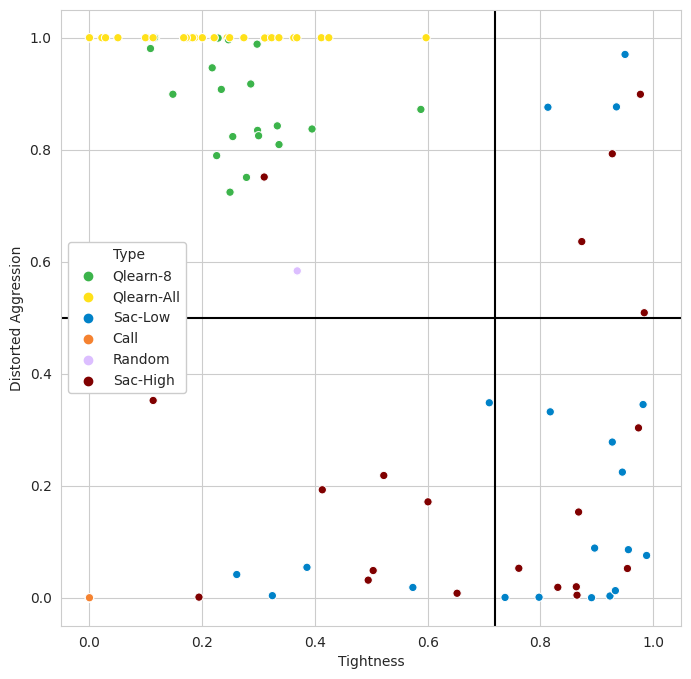
\includegraphics[width=0.8\linewidth]{Results/figures/traditional_scatterplot_Type.png}
\caption{Aggression and Tightness, colored by agent type}
\label{AggTightAgentType}
\end{figure}

\begin{figure}[H]
\centering
\subcaptionbox{
    Ranked by TrueSkill
}{
    
\includegraphics[width=0.45\linewidth]{Results/figures/placeholder.png}
}
\subcaptionbox{
    Ranked by Mean
}{
    
\includegraphics[width=0.45\linewidth]{Results/figures/placeholder.png}
}
\subcaptionbox{
    Ranked by Median
}{
    
\includegraphics[width=0.45\linewidth]{Results/figures/placeholder.png}
}
\subcaptionbox{
    Ranked by 20-Percentile
}{
    
\includegraphics[width=0.45\linewidth]{Results/figures/placeholder.png}
}
\caption{Agent evolution over time by type and rank [LINE GENERATIONPLOT]}
\label{AgentGenerations}
\end{figure}

\begin{code}
    - convergence speed
    - skill cap
\end{code}

\section{Populations}
\begin{table}[H]
\centering
\begin{tabular}{|| c | c | c | c | c | c ||} 
 \hline
 Rank & TrueSkill & Mean & Median & 20-Percentile \\ [0.5ex] 
 \hline\hline
 \todo{wrong table}
   1 &   Qln8-Cl &   QlnA-Cl &   QlnA-Cl &       QlnA-Rn \\
   2 &   Qln8-Cl &   QlnA-Cl &   Qln8-Cl &       QlnA-Cl \\
   3 &   QlnA-Rn &   QlnA-Cl &   Qln8-Cl &       Qln8-Cl \\
   4 &   Qln8-Cl &   QlnA-Cl &   Qln8-Cl &       Qln8-Cl \\
   5 &   QlnA-Rn &  AllAg-Cl &   QlnA-Rn &       QlnA-Cl \\
   6 &   Qln8-Cl &   QlnA-Rn &   QlnA-Rn &       Qln8-Cl \\
   7 &   QlnA-Cl &   QlnA-Rn &   Qln8-Cl &       Qln8-Cl \\
   8 &   Qln8-Cl &   QlnA-Rn &   Qln8-Cl &       Qln8-Cl \\
   9 &   Qln8-Cl &   QlnA-Rn &   Qln8-Cl &      AllAg-Cl \\
  10 &   QlnA-Rn &   QlnA-Rn &   Qln8-Cl &       Qln8-Cl \\
  11 &   QlnA-Rn &   QlnA-Cl &   QlnA-Cl &       QlnA-Rn \\
  12 &   Qln8-Cl &   QlnA-Cl &   QlnA-Rn &       QlnA-Rn \\
  13 &   QlnA-Cl &   Qln8-Cl &   QlnA-Rn &      AllAg-Cl \\
  14 &  AllAg-Cl &   QlnA-Rn &  AllAg-Cl &       QlnA-Rn \\
  15 &  AllAg-Cl &  AllAg-Cl &   QlnA-Rn &       QlnA-Cl \\
  16 &   QlnA-Cl &   Qln8-Cl &   Qln8-Cl &      AllAg-Cl \\
  17 &   QlnA-Rn &   Qln8-Cl &   QlnA-Cl &       QlnA-Rn \\
  18 &   QlnA-Rn &   Qln8-Cl &   QlnA-Cl &      AllAg-Cl \\
  19 &  AllAg-Cl &   Qln8-Cl &   QlnA-Cl &       QlnA-Cl \\
  20 &   QlnA-Cl &   Qln8-Cl &   QlnA-Rn &       QlnA-Rn \\ [1ex] 
 \hline
\end{tabular}
\label{DivisionRankings}
\caption{Agent division of the top 20 agents according to each metric}
\end{table}

\begin{figure}[H]
\centering
    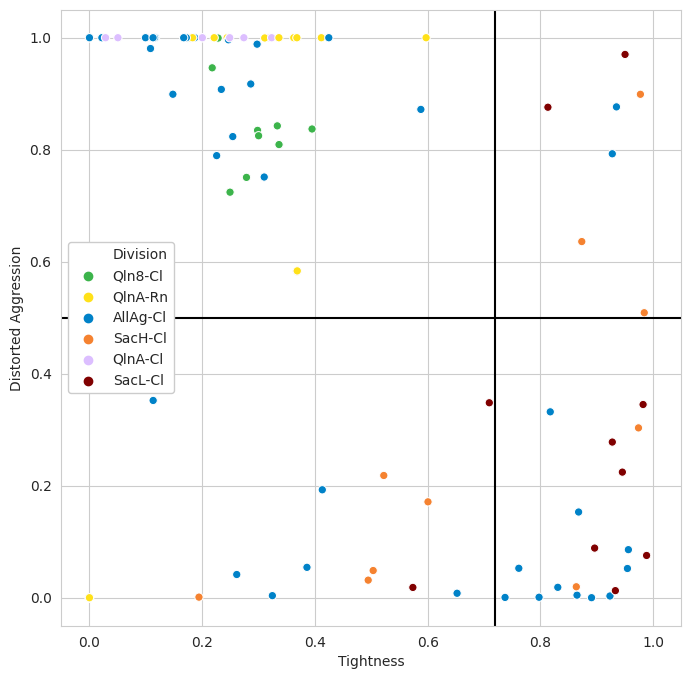
\includegraphics[width=0.8\linewidth]{Results/figures/traditional_scatterplot_Division.png}
\caption{Aggression and Tightness, colored by division}
\label{AggTightDivision}
\end{figure}

\begin{code}
    - discussion (note that mixed league had less games per agent, but same compute)
\end{code}

\begin{figure}[H]
\centering
\subcaptionbox{
    Ranked by TrueSkill
}{
    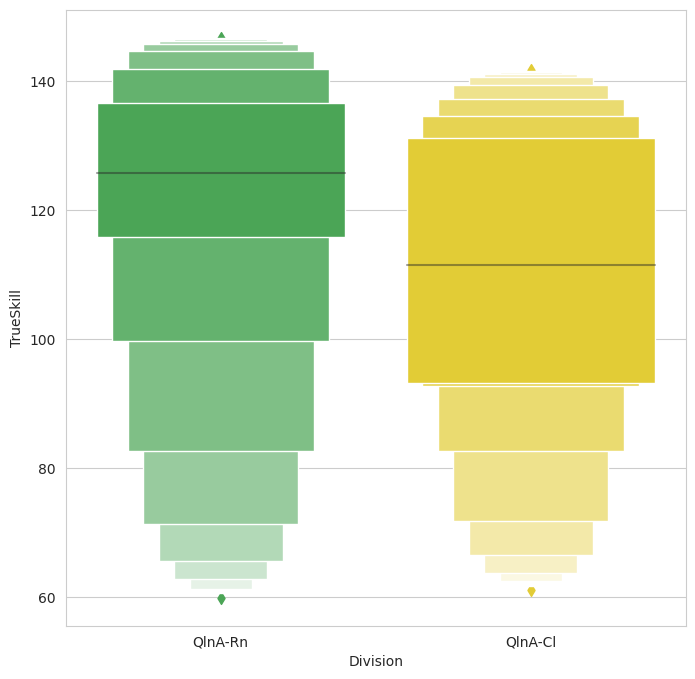
\includegraphics[width=0.45\linewidth]{Results/figures/matchupdistTrueSkill.png}
}
\subcaptionbox{
    Ranked by Mean
}{
    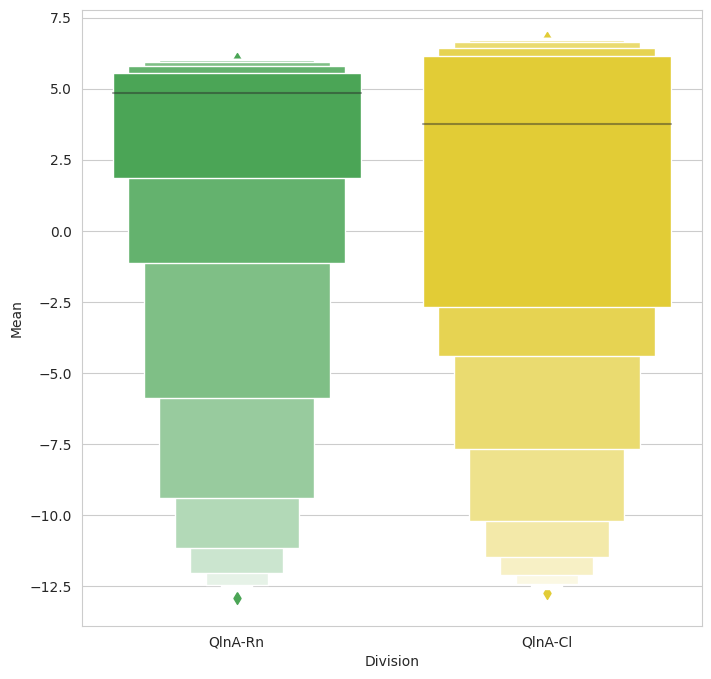
\includegraphics[width=0.45\linewidth]{Results/figures/matchupdistMean.png}
}
\subcaptionbox{
    Ranked by Median
}{
    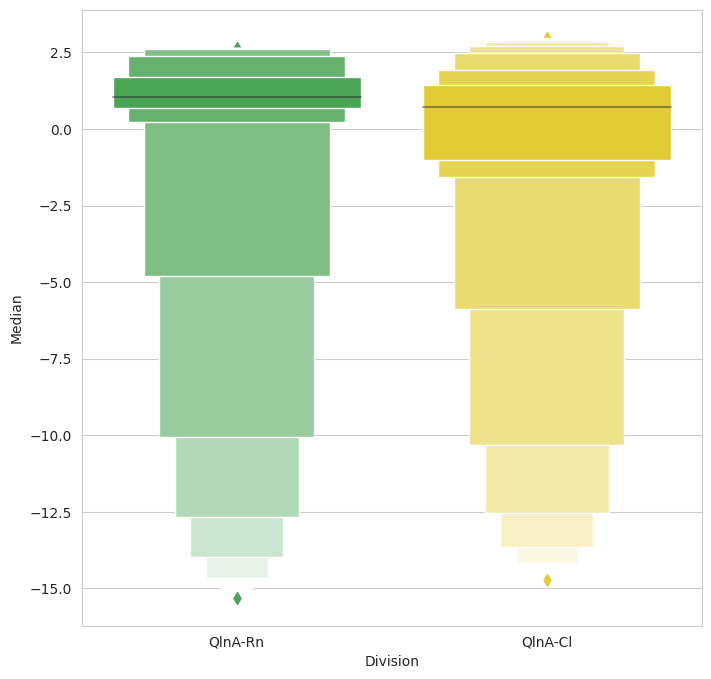
\includegraphics[width=0.45\linewidth]{Results/figures/matchupdistMedian.png}
}
\subcaptionbox{
    Ranked by 20-Percentile
}{
    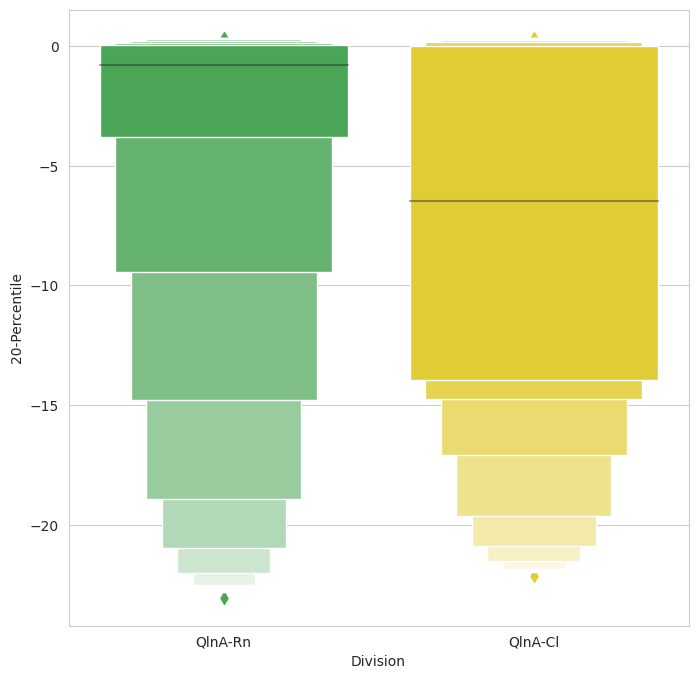
\includegraphics[width=0.45\linewidth]{Results/figures/matchupdist20-Percentile.png}
}
\caption{Agent distribution by matchup type}
\label{MatchupDistribution}
\end{figure}

\begin{table}[H]
\centering
\begin{tabular}{|| c | c ||} 
 \hline
 Division & Kendall's Tau \\ [0.5ex] 
 \hline\hline
     Qln8-Cl & 1 \\
     QlnA-Cl & 1 \\
     SacL-Cl & 1 \\
     SacH-Cl & 1 \\
     AllAg-Cl & 1 \\
     QlnA-Rn & 1 \\ [1ex] 
 \hline
\end{tabular}
\label{DivisionInternalExternal}
\caption{Kendall's Tau between internal division rankings and PermaEval}
\end{table}

\begin{code}
    - discussion
    - how overfitted are they
    - are internal ratings representative of external ratings?
\end{code}

%- [TABLE,]
%    - exploiters -> ? where expected winner lost with highest negative